\section{Mixed Precision Quantization-aware}

% \begin{frame}{Uniform Bit Resolution Limitation}
%     % Even though eliminating outlier values can lead to better performance, 

    
%     D
    
    

    
% \end{frame}

\begin{frame}{Mixed-precision Architecture}
\begin{itemize}
    \item Uniformly assigning bit resolution along layers may not be optimal %in cases where mixed precision is allowed. 
    \item Different layers varying in redundancy and contribute differently to the final performance.
    \item Identifying the bit-precision tolerance of each layer allows different computation rate~\footnote{\scriptsize Giamougiannis, G., Tsakyridis, A., Moralis-Pegios, M., Pappas, C.,
      \textbf{Kirtas, M.}, Passalis, N., Lazovsky, D., Tefas, A. and Pleros, N.,
      2023.\href{https://www.degruyter.com/document/doi/10.1515/nanoph-2022-0423/html}{ Analog
      nanophotonic computing going practical: silicon photonic deep learning
      engines for tiled optical matrix multiplication with dynamic precision.} Nanophotonics.}
\end{itemize}
    \begin{center}
        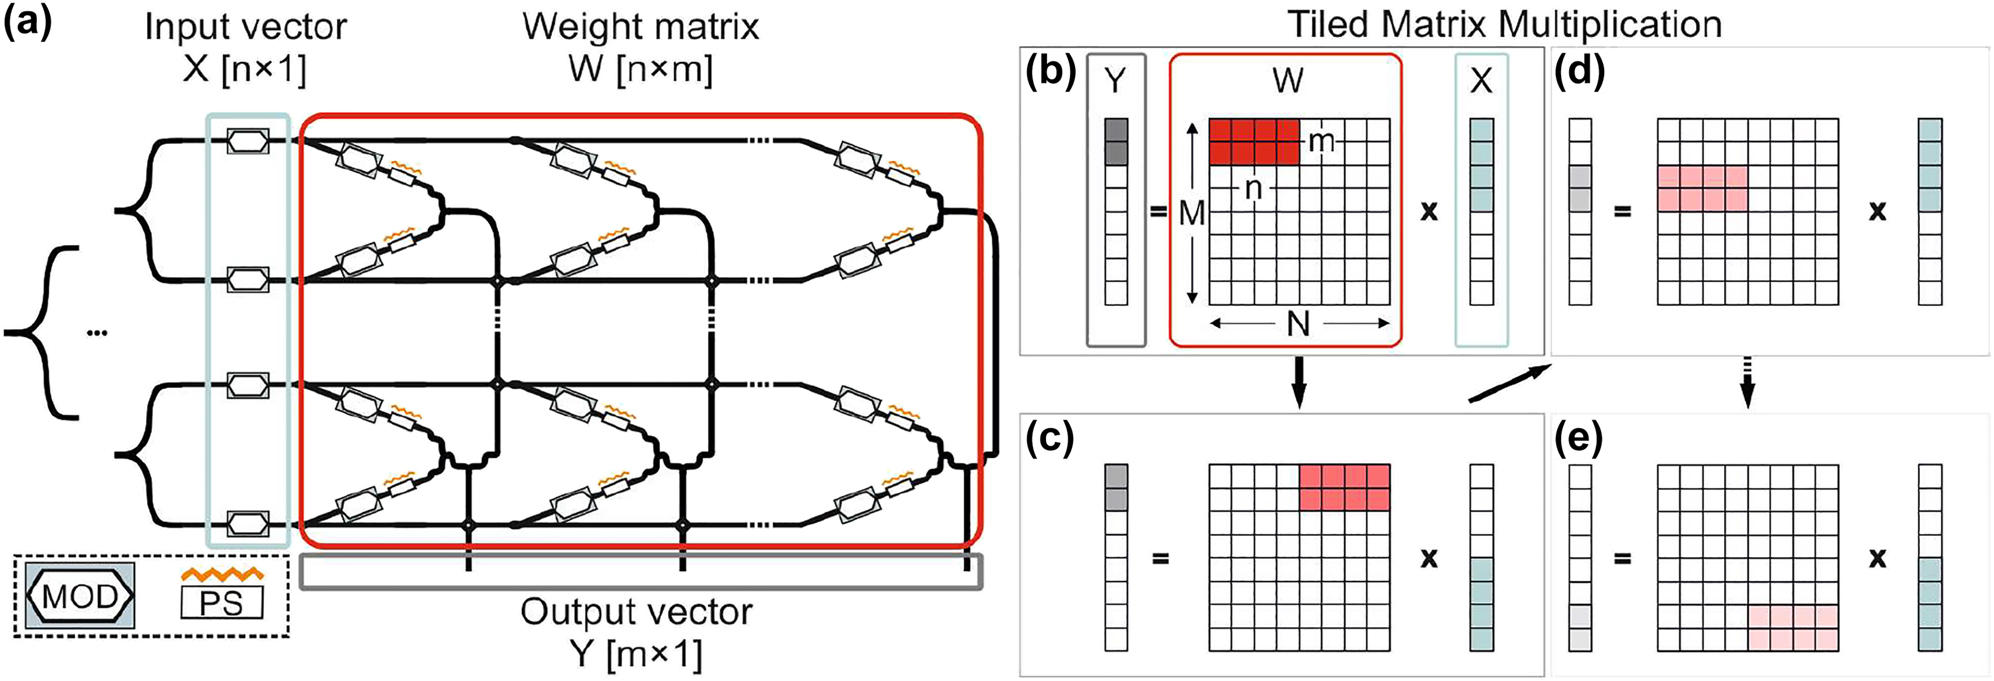
\includegraphics[width=0.8\textwidth]{sections/3_mixedquant/imgs/j_nanoph-2022-0423_fig_001.jpg}    
    \end{center}
    % of the linear operations during inference
\end{frame}

\begin{frame}{Mixed-precision Benefits}
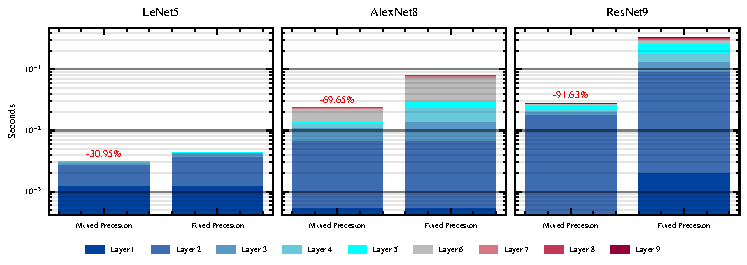
\includegraphics[width=\textwidth]{sections/3_mixedquant/imgs/exe_time.pdf}

\begin{itemize}
    \item Leads to execution time savings
    \item Lower latency
    \item Energy savings
    \item Better scalability
\end{itemize}
    
\end{frame}


\begin{frame}{Proposed Method} 
  The proposed \textbf{stochastic}, \textbf{architecture-agnostic}, \textbf{mixed-precision quantization-aware} training scheme: 
\begin{enumerate}
    \item Formalizes mixed precision quantization-aware training.
    \item \textbf{Gradually bit resolution reduction among layers.} 
    % \item Unlocks the novel mixed precision capabilities of PNNs
    \end{enumerate}
    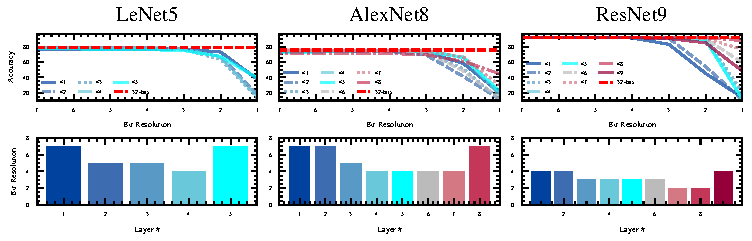
\includegraphics[width=\textwidth]{sections/3_mixedquant/imgs/dynamic_plot.pdf}
    Exploiting that the intermediate layers are more tolerant to quantization errors.
\end{frame}

\begin{frame}{Mixed Precision Quantization Formulation}
	Conceptually, the proposed method is motivated by the roulette wheel selection
  approach that is widely used in genetic algorithms.
  \begin{center}
   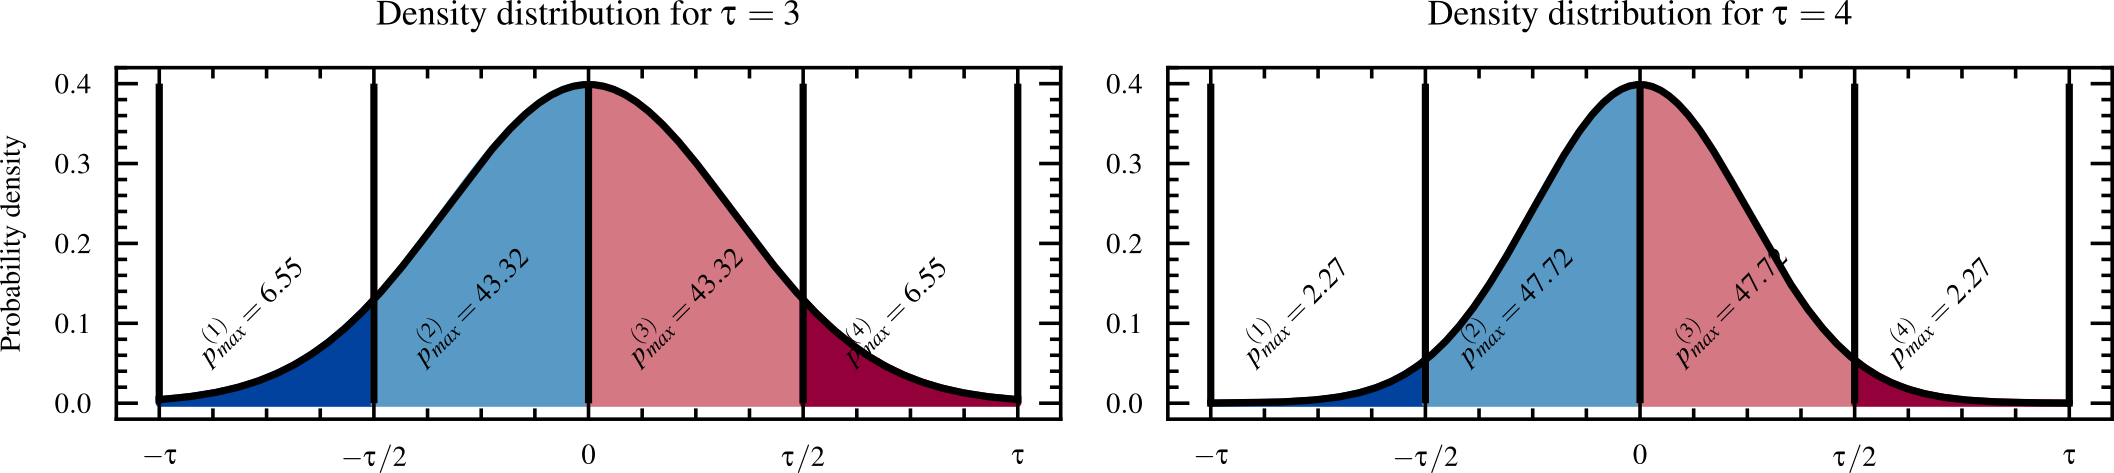
\includegraphics[width=\textwidth]{sections/3_mixedquant/imgs/gaussian_distributions.png }
  \end{center}
   \textbf{Attaches a higher probability for lower bit resolutions to intermediate layers than to outer ones following a normal distribution.}
\end{frame}



% \begin{frame}{}

% Maximum probability for a layer to reduce its bit resolution is assigned based on its position.
% \end{frame}

\begin{frame}{Maximum Probability of Each Layer}
  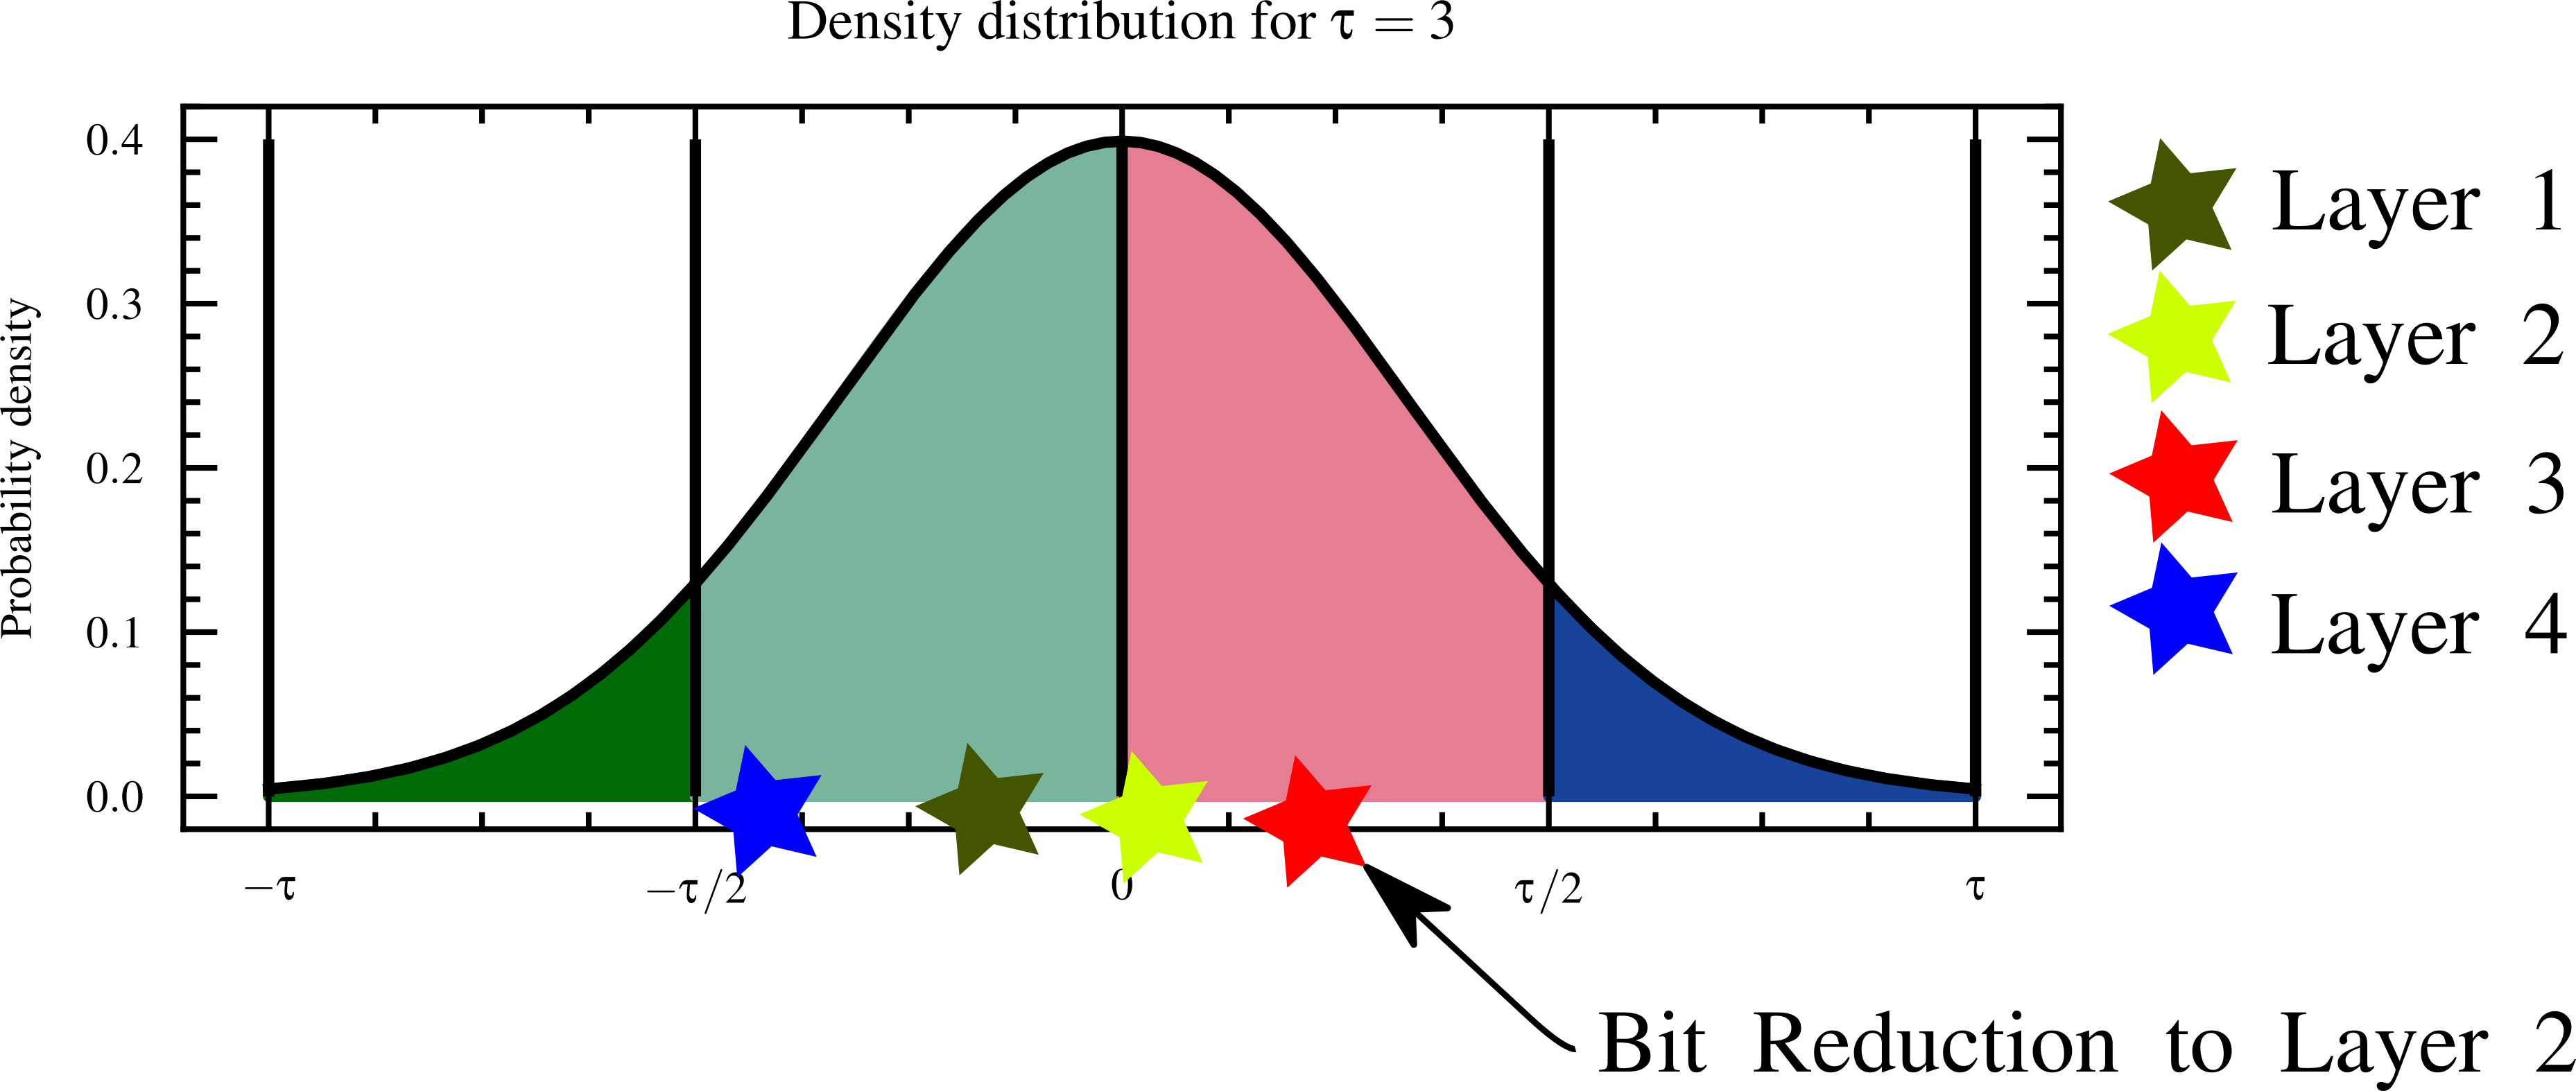
\includegraphics[width=0.8\textwidth]{sections/3_mixedquant/imgs/max_propability.png}
  
At every epoch \(t \in [0, T]\), such values as the number of layers \(\bm{u} \in
\mathbb{R}^{n}\) are drawn from the Gaussian distributions,
\begin{equation}
  \bm{u} \sim \mathcal{N}_{n}(\mu, \sigma)\in \mathbb{R}^{n},
\end{equation}
{\scriptsize  where \(n \in \mathbb{N}\) denotes the number of layers,
\(\mu \in \mathbb{R}\) and \(\sigma \in \mathbb{R}\) define the mean and
standard deviation of the Gaussian distributions, respectively.}

  
  % When the layer is at its maximum probability, a bit reduction occurs if the point \(u^{(i)}_t \sim \mathcal{N}(\mu, \sigma)\), drawn from the Gaussian distribution, is within the range
  % \(u^{(i)}_t \in [a^{(i)},a^{(i+1)})\), with \(p^{(i)}_{max, t} \in \mathbb{R}\) probability at
  % \(t\)-th timestep.
  % \begin{equation}
  %   r_{t+1}^{(i)}=\left\{
  %     \begin{array}{ll}
  %       % r_t^{(i)} & \text{if } r_t^{(i)} \leq r_{min},\\
  %   max\{r_{min}, r_t^{(i)} - r_{step}\} &  \text{if } a^{(i)} \leq u^{(i)}_t  \leq a^{(i+1)}\\
  %   r_{t}^{(i)} & \text{otherwise}.
  %     \end{array}
  %   \right .
  % \end{equation}

\end{frame}

\begin{frame}{The need for Gradual Reduction}
\begin{itemize}
    \item Providing the maximum possibility \(p^{(i)}_{max} \in \mathbb{R}\) results in low precisions in first few epochs of the training.
      \item The quantization noise will be high in the early in training where the network is unstable and not close to their convergent stage.
  \end{itemize}
  \begin{center}
  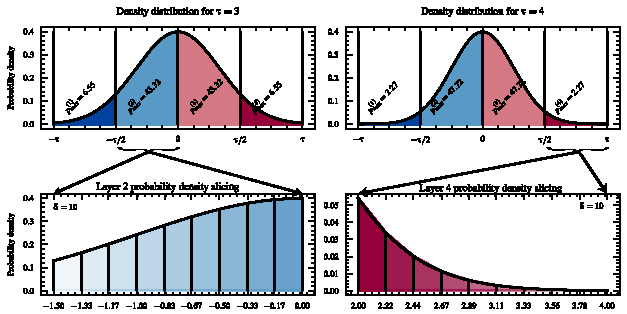
\includegraphics[width=0.8\textwidth]{sections/3_mixedquant/imgs/proposed_explained.pdf}  
  \end{center}
  A gradual bit reduction is proposed, achieved by uniformly slicing the maximum possible range of each layer.

%   \begin{itemize}
%   \item The proposed method gradually increase each layer probability until the its
%   maximum.
%   \item This is ac
%   \item  A divisor value is introduced to slice the maximum available range
%   of  \([a^{(i)},a^{(i+1)})\) in  \(\delta \in \mathbb{N}_{+}\) uniform slices
% \end{itemize}

%     \begin{enumerate}
%         \item The \textit{active} range is increased either until its maximum available range, which is equivalent to the maximum probability density
%         \item The point drawn from the Gaussian distribution \(u^{(i)}_t \sim \mathcal{N}(\mu, \sigma)\) drops within the active range \(u^{(i)}_t \in \bm{\Delta}^{(i)}_{j_t^{(i)} }\).
%     \end{enumerate}
%   \begin{equation}
% \begin{aligned}
%   \bm{\Delta}^{(i)} = [&a^{(i)}, a^{(i)} + \frac{a^{(i+1)} -
%   a^{(i)}}{\delta}, \ldots, \\
%   & a^{(i)} + \frac{(\delta-1)\left(a^{(i+1)} -
%         a^{(i+1)}\right)}{\delta}, a^{(i+1)} ] \in \mathbb{N}^{\delta}_{+},
% \end{aligned}
% \end{equation}
% {\scriptsize where the \(\bm{\Delta}^{(i)} \in \mathbb{N}^{\delta}_{+}\) is
%   called \textit{active} range of \(i\)-th 
% layer. }
\end{frame}

% \begin{frame}{Title}
%  The \(j_t^{(i)}  \in [1, \ldots, \delta]\)
% defines the epoch passed either from the start of training or from the last bit
% reduction. Therefore, at every training epoch \(t\) that the drawn value is not
% within the active range, \(u^{(i)}_{t} \notin \bm{\Delta}^{(i)}_{j_t^{(i)} }\), the
% \(j_t^{(i)} \in [1, \ldots, \delta]\) increased by a unit \(j_{t+1}^{(i)} =min\{j_{t}^{(i)} ,
% \delta\}\) if it is not equal to \(\delta \in \mathbb{N}_{+}\), increasing in this way the active
% range \(\bm{\Delta}^{(i)}_{j+1}\) by another a slice, expreseed by:   
% \begin{equation}
%     \bm{\Delta}^{(i)}_{j_{t}^{(i)}}= \left\{ \begin{array}{ll}
%          \left[a^{(i)} + \frac{(\delta-j^{(i)}_t)(a^{(i+1)} - a^{(i)})}{\delta}, a^{(i+1)}\right) & a^{(i)} \geq 0 \\[10pt]
%          \left[a^{(i)} + \frac{j^{(i)}_t(a^{(i+1)} - a^{(i)})}{\delta}, a^{(i+1)}\right) & \text{otherwise}. \\
%     \end{array}
%     \right.
%   \end{equation}
% \end{frame}

\begin{frame}{Smooth Bit Reduction}
% 	The two cases define the probability increase for both sides of the normal
% distributions, as shown in the second row of Figure~\ref{fig:proposed_exp}. If
% the range of the layer is on the negative side of the distribution, then the
% probability increases by unlocking the next slice on its right. Otherwise, if
% the layer is on the positive side of the distribution, the probability is
% increased by decreasing the lower bound to unlock another slice. In both cases,
% the probability of the \(i\)-th layer performing a bit reduction is increased,
% \(p^{(i)}_{j+1} \geq p^{(i)}_{j}\).  In the case where \(u^{(i)}_t \in
% \bm{\Delta}_{j}^{(i)}\), the active range is reset to its minimum,
% \(\bm{\Delta}^{(i)}_{j=1}\), and the method performs a bit reduction according
% to \(r^{(i)}_{t} = max\{r^{(i)}_{t-1} - r_{step}, r_{min}\}\).

The proposed method allows \textbf{smoothly increase the quantization error},
ensuring that the \textbf{noise is first introduced to more tolerant layers}. 
\begin{center}
    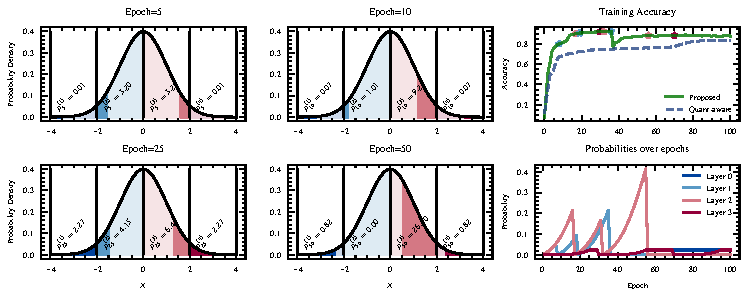
\includegraphics[width=\textwidth]{ sections/3_mixedquant/imgs/mnist_pos.pdf}
\end{center}
\end{frame}

% \begin{frame}{Probability of bit reduction}
% The probability of the \(i\)-th layer to reduce its precision by \(r_{step} \in \mathbb{N}_{+}\) bits at \(t\)-th epochs is given by:  
% \begin{equation}
%     p^{(i)}_{t} = \left\{
%     \begin{array}{ll}
%     min\left\{p^{(i)}_{max},  \frac{1}{\sqrt{2\pi}}\int_{\bm{\Delta}_{j_t^{(i)}}}e^{-z^2/2}dz\right\} & \text{if } b_{t}^{(i)} < b_{max},\\[10pt]
%     0 & \text{otherwise},
%     \end{array}
%      \right. 
% \end{equation}
% where \(j\) is calculated at every epoch \(t\) as:
% \begin{equation}
%      j_{t+1}^{(i)}=\left\{
%     \begin{array}{ll}
%     1 &  \text{if } u_{t} \in \bm{\Delta}_{j_t^{(i)}},\\
%     min\{j_t^{(i)} + 1, \delta\} & \text{otherwise},
%     \end{array}
%   \right. 
% \end{equation}
% with \(\{j_1^{(i)}=1 \mid 1 < i < n \}\). 
% \end{frame}

% \begin{frame}
% 	In this work, we used the default hyperparameter values for all experimental
% evaluation cases. More specifically, we empirically propose using a normal
% distribution with 0 mean and variance equal to 1,
% \(\mathcal{N}(\mu=0,\sigma=1)\), while setting \(\tau=3\). The gradual increment
% of probability for bit reduction of each layer depends on \(\delta\), and in
% turn, we set equal to \(\delta=M/4\), where \(M \in \mathbb{N}\) is the number of epochs.
% Finally, the bit reduction step is set to \(r_{step}=2\). It should be mentioned
% that the proposed method is presented for an even number of layers for
% simplicity, but it can be used straightforwardly for an odd number of layers
% simply by shifting the normal distribution right or left.    

% \end{frame}

% \begin{frame}{Experimental Evaluation: 4-Layer MLP in MNIST}
% 	\begin{table}[ht]
%     \resizebox{0.85\linewidth}{!}{
% \begin{tabular}{l|ccc}
%     \toprule
%          \textbf{Avg. Bits} &  \textbf{Post Quantization} & \textbf{Quant. Training} & \textbf{Proposed} \\
%      \midrule
%      \multicolumn{4}{c}{\textbf{Photonic Sinusoidal} \hspace{0.1cm} \( (\mathit{93.35\pm{0.23}}) \)}\\
%      \midrule
%      7 & $15.97\pm{2.95}$ & $92.77\pm{0.19}$ & $\bm{93.00\pm{0.09}}$\\
%      6 & $15.38\pm{2.39}$ & $92.57\pm{0.26}$ & $\bm{92.87\pm{0.20}}$\\
%      5 & $15.39\pm{2.32}$ & $92.40\pm{0.21}$ & $\bm{92.48\pm{0.20}}$\\
%      4 & $15.35\pm{5.11}$ & $91.95\pm{0.30}$ & $\bm{92.19\pm{0.22}}$\\
%      3 & $15.35\pm{2.37}$ & $85.35\pm{3.45}$ & $\bm{89.77\pm{0.66}}$\\
%      2 & $12.80\pm{1.02}$ & $64.78\pm{3.30}$ & $\bm{73.61\pm{5.85}}$\\
%      \midrule
%      \multicolumn{4}{c}{\textbf{Photonic Sigmoid} \hspace{0.1cm} \( \mathit{(92.10 \pm{0.52})} \)}\\
%      \midrule
%      7 & $86.31\pm{7.78}$ & $92.14\pm{0.18}$ & $\bm{92.44\pm{0.14}}$\\
%      6 & $82.09\pm{5.97}$ & $92.29\pm{0.37}$ & $\bm{92.37\pm{0.34}}$\\
%      5 & $82.16\pm{1.25}$ & $92.07\pm{0.32}$ & $\bm{92.12\pm{0.15}}$\\
%      4 & $70.82\pm{7.24}$ & $91.14\pm{0.22}$ & $\bm{91.68\pm{0.32}}$\\
%      3 & $54.94\pm{7.13}$ & $89.31\pm{0.44}$ & $\bm{89.35\pm{0.64}}$\\
%      2 & $28.64\pm{1.92}$ & $64.36\pm{2.95}$ & $\bm{66.10\pm{2.88}}$\\ 
%      \bottomrule
% \end{tabular}}
% \end{table}
% \end{frame}


% \begin{frame}{Experimental Evaluation: }
%   \begin{table}[ht]
% % \caption{Evaluating the proposed method on the CIFAR10 dataset using ResNet8.
% %   The table reports the average evaluation accuracy and standard deviation over
% %   5 runs. }
%     \centering
%     \resizebox{0.85\linewidth}{!}{
%       \begin{tabular}{l|ccc}
%         \toprule
%         \textbf{Bits} &  \textbf{Post Quantization} & \textbf{Quant. Training} & \textbf{Proposed} \\
%         \midrule
%         \multicolumn{4}{c}{\textbf{Photonic Sinusoidal} \hspace{0.1cm} \( (\mathit{73.14 \pm{0.60}}) \)}\\
%         \midrule
%         7 & $10.00\pm{0.00}$ & $67.56\pm{1.13}$ & $\bm{69.69\pm{0.65}}$\\
%         6 & $10.00\pm{0.00}$ & $67.07\pm{2.13}$ & $\bm{70.01\pm{0.79}}$\\
%         5 & $10.00\pm{0.00}$ & $67.87\pm{2.36}$ & $\bm{68.48\pm{0.85}}$\\
%         4 & $10.00\pm{0.00}$ & $64.20\pm{1.06}$ & $\bm{65.69\pm{2.30}}$\\
%         3 & $10.00\pm{0.00}$ & $53.71\pm{1.53}$ & $\bm{54.81\pm{5.43}}$\\
%         \midrule
%         \multicolumn{4}{c}{\textbf{Photonic Sigmoid} \hspace{0.1cm} \( \mathit{(63.31 \pm{0.63})} \)}\\
%         \midrule
%         7 & $10.00\pm{0.00}$ & $58.43\pm{2.14}$ & $\bm{62.09\pm{0.95}}$\\
%         6 & $10.00\pm{0.00}$ & $61.38\pm{2.32}$ & $\bm{62.26\pm{1.46}}$\\
%         5 & $10.00\pm{0.00}$ & $57.83\pm{1.00}$ & $\bm{61.08\pm{1.70}}$\\
%         4 & $10.00\pm{0.00}$ & $48.14\pm{2.33}$ & $\bm{52.62\pm{0.92}}$\\
%         3 & $10.00\pm{0.00}$ & $31.94\pm{3.55}$ & $\bm{39.92\pm{2.03}}$\\
%         \bottomrule
%       \end{tabular}}
%     \label{tab:2_2_cifar_exp}
%   \end{table}
% \end{frame}

\begin{frame}{ResNet8 in CIFAR10 Inference Time}
  \begin{figure}
    \centering
    \begin{subfigure}{.6\textwidth}
      \centering
      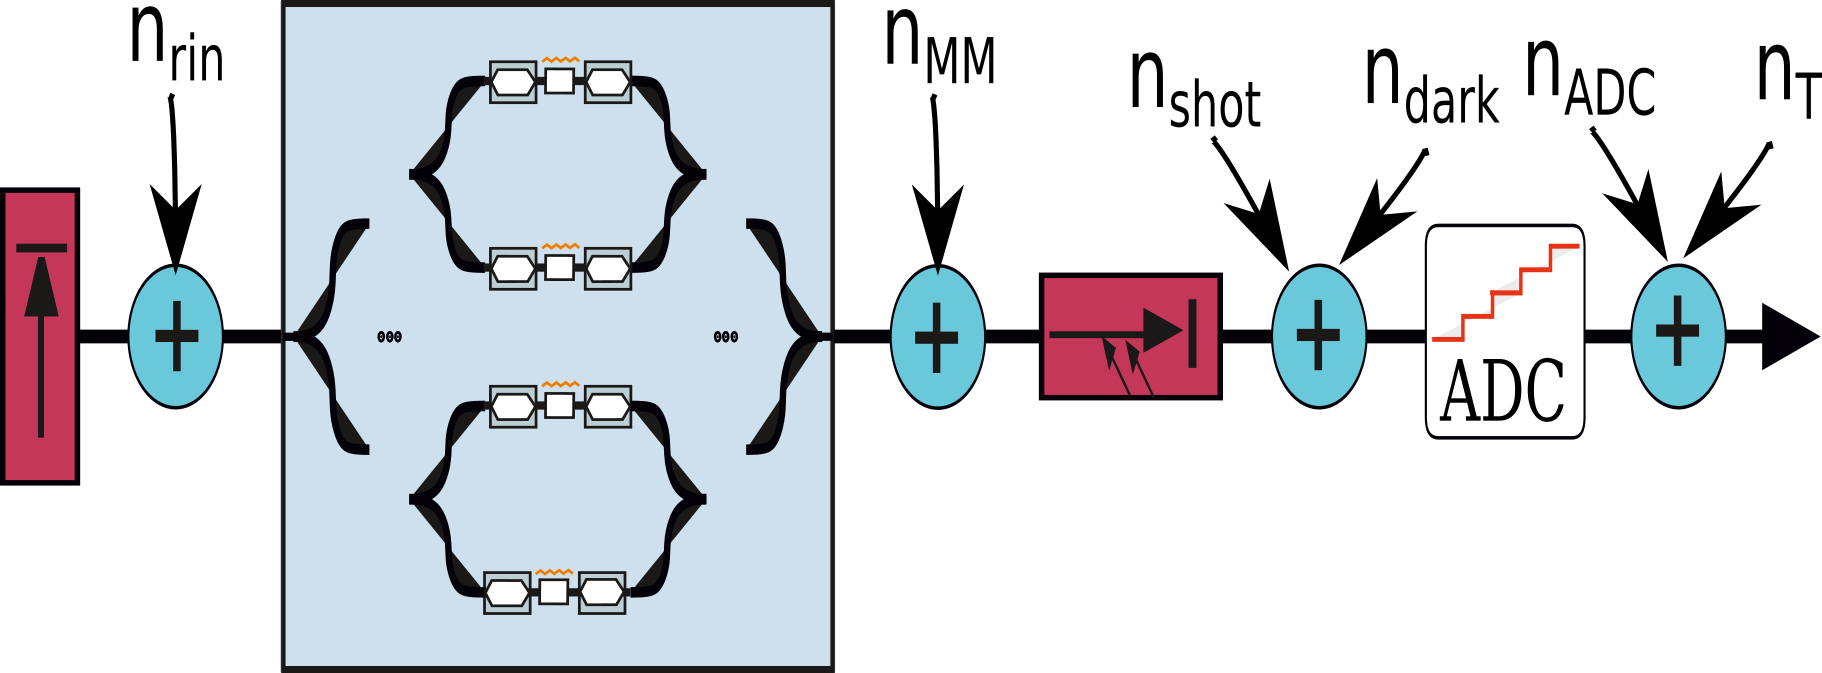
\includegraphics[width=0.9\textwidth]{sections/3_mixedquant/imgs/path1638.png}
      \caption{}
      \label{fig:noise_sources}
    \end{subfigure}\hfill
    \begin{subfigure}{.4\textwidth}
      \centering
      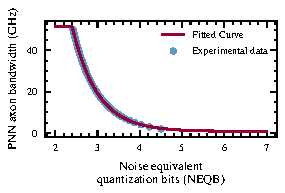
\includegraphics[width=0.8\textwidth]{sections/3_mixedquant/imgs/exe_time_fit.pdf}
      \caption{}
      \label{fig:evel_exe_time}
    \end{subfigure}
    % \caption {(a) PNN noise sources breakdown,  (b) PNN axon bandwidth versus equivalent bit resolution}
    \label{fig:background}
  \end{figure}
  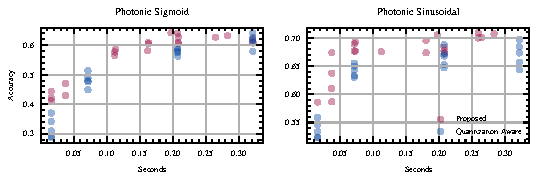
\includegraphics[width=\textwidth]{
    sections/3_mixedquant/imgs/exec_time_cifar10.pdf}      
\end{frame}


% \begin{frame}{Experimental Evaluation: RNN in FI2010}
% 	\begin{table}[ht]
% % \caption{Evaluating the proposed method on the FI2010 dataset using RNN. The
% %   table reports the average Cohen kappa metric and standard deviation on five
% %   splits in 3 evaluation runs.}
%     \centering
%     \resizebox{0.9\linewidth}{!}{
% \begin{tabular}{l|ccc}
%     \toprule
%          \textbf{Bits} &  \textbf{Post Quantization} & \textbf{Quant. Training} & \textbf{Proposed} \\
%      \midrule
%      \multicolumn{4}{c}{\textbf{Photonic Sinusoidal} \hspace{0.1cm} \( (\mathit{0.1637\pm{0.0061}}) \)}\\
%      \midrule
%      7 & $0.1469\pm{0.0032}$ & $0.1694\pm{0.0019}$ & $\bm{0.1730\pm{0.0006}}$\\
%      6 & $0.1433\pm{0.0056}$ & $0.1682\pm{0.0072}$ & $\bm{0.1724\pm{0.0003}}$\\
%      5 & $0.1400\pm{0.0057}$ & $0.1659\pm{0.0080}$ & $\bm{0.1703\pm{0.0009}}$\\
%      4 & $0.1391\pm{0.0159}$ & $0.1602\pm{0.0033}$ & $\bm{0.1656\pm{0.0032}}$\\
%      3 & $0.0388\pm{0.0058}$ & $0.1411\pm{0.0075}$ & $\bm{0.1427\pm{0.0067}}$\\
%      \midrule
%      \multicolumn{4}{c}{\textbf{Photonic Sigmoid} \hspace{0.1cm} \( \mathit{(0.1395\pm{0.0047})} \)}\\
%      \midrule
%      7 & $0.1355\pm{0.0036}$ & $0.1375\pm{0.0016}$ & $\bm{0.1392\pm{0.0044}}$\\
%      6 & $0.1355\pm{0.0009}$ & $0.1370\pm{0.0050}$ & $\bm{0.1398\pm{0.0010}}$\\
%      5 & $0.1391\pm{0.0026}$ & $0.1364\pm{0.0030}$ & $\bm{0.1404\pm{0.0005}}$\\
%      4 & $0.1124\pm{0.0035}$ & $0.1372\pm{0.0046}$ & $\bm{0.1388\pm{0.0013}}$\\
%      3 & $0.0871\pm{0.0017}$ & $0.1223\pm{0.0004}$ & $\bm{0.1226\pm{0.0007}}$\\
%      \bottomrule
% \end{tabular}}
% \end{table}
% \end{frame}

\begin{frame}{Publications}
\begin{itemize}
    \item Main Journal Publications
    \begin{itemize}
        \item {\scriptsize\textbf{Kirtas, M.}, Passalis, N., Oikonomou, A., Moralis-Pegios, M.,
      Giamougiannis, G., Tsakyridis, A., Mourgias-Alexandris, G., Pleros, N. and Tefas, A., 2023. \href{https://link.springer.com/article/10.1007/s00521-023-08848-8}{Mixed-precision quantization-aware training for photonic neural networks}. Neural Computing and Applications, Springer}
    \end{itemize}
    \item Main Conference Publications 
        \begin{itemize}
        \item {\scriptsize \textbf{Kirtas, M.}, Passalis, N., Oikonomou, A., Moralis-Pegios, M.,
      Giamourgiannis, G., Tsakyridis, A., Mourgias-Alexandris, G., Pleros, N. and Tefas, A., 2023, September.
      \href{https://ieeexplore.ieee.org/document/10285966}{Quantization-Aware Training for Mixed Precision Photonic Neural Networks.} In 2023 IEEE 33rd International Workshop on Machine Learning for Signal Processing (MLSP)} 
    \end{itemize}
\end{itemize}
\end{frame}
